
\chapter{Experimental Study}

\section{Data}

\subsection{Explaining the data}

The dataset used in this thesis is the \quotedblbase{}Corpus of English Translated Texts and Originals (CETTO)’’ (Doherty et al., 2021), available on Zenodo: \href{https://zenodo.org/record/5596238}{zenodo.org/record/5596238}. 
Out of the single-source monolingual data sets, only mono\_de\_en and mono\_es\_en were used.
This data was split into 2 sections: DE-EN and ES-EN.
Each data set consists of 42.260 English texts, of which 21.130 translated texts and 21.130 non-translated texts.

Both translated and original texts are taken from diverse genres, such as fiction, non-fiction, news articles, and technical documents, to ensure a representative sample of English texts and specific vocabulary. 

\subsection{Preprocessing Procedure}

Before implementing the classification models, the data set needs to be processed in advance to ensure the optimal performance of both feature engineering and feature learning approaches. The pre-processing steps were done with a pre-trained tokenizer \cite{huggingfaces}. 

Import tokenizer :
\begin{lstlisting}[language=Python]
    tokenizer = BertTokenizer.from_pretrained(name)
\end{lstlisting}

The lowercase texts undergo tokenization with the usage of WordPiece and a 30,000-sized vocabulary. Subsequently, the model's inputs are structured in the following manner:

\begin{center}
    [CLS] First Sentence [SEP] Second Sentence [SEP]
\end{center}

There exists a 50\% probability that the First Sentence and Second Sentence are sequential sentences in the original body of text, the corpus. In other scenarios, the chosen sentence might be a random selection from the corpus. Here, a sentence is defined as a contiguous span of text, generally exceeding a single sentence in length. The sole requirement for these "sentences" is that their combined length should not surpass 512 tokens.

It is crucial to note that the term "sentence" as utilized here, does not strictly refer to a single sentence in traditional syntactic terms, but rather to a continuous stretch of text which might be lengthier than a conventional phrase. Only one condition is a prerequisite, namely the fact that the combined size of two ”sentences” must not be over 512 tokens.

The outlined specifications for the masking procedure for each sentence are as follows:

\begin{itemize}
    \item Fifteen percent (15\%) of the tokens within a sentence are subjected to masking.
    \item Among the masked tokens, eighty percent (80\%) are substituted with the [MASK] token.
    \item The masked tokens are switched with randomly selected tokens that are not the same as the original ones in 10\% of the cases
    \item The remaining ten percent (10\%) of the masked tokens remain unchanged.
\end{itemize}

Extract input\_ids, attention\_masks and token\_type\_ids:

\begin{lstlisting}[language=Python]
    for text in X:
        out_dict = tokenizer.encode_plus(
            text,                  # Text for encoding
            truncation = True,
            max_length = max_len,
            add_special_tokens = True, # Adding '[SEP]', '[CLS]'
            padding = 'max_length',
            return_tensors = 'pt',     # This line returns a tensor.
            return_attention_mask = True,
            return_token_type_ids=True,
        )
\end{lstlisting}

After this operation, we construct a DataLoader with TensorDataset(input\_ids, attention\_masks, token\_type\_ids, labels), batch\_size and shuffle (boolean value).


\section{Results}

In the process of obtaining the best accuracy, I initially passed all the texts through the BERT model which was set in test mode, that is, backward() was not done through the network. The [CLS] output for a text was a tensor with a size of 768. Then I trained several Neural Networks (NN) to see which ones presented the best accuracy. The best models from Experiment 1 were used further, in Experiment 2.

\subsection{Experiment 1}

Experiment 1 consisted of finding the best model for fine-tuning. The tested models exhibited variations in both the type and quantity of layers employed, as well as various activation functions. The number of epochs was the same for all, this being 50. The learning rate took values from the following array 
$[4*10^{-5}, 4*10^{-4}, 2*10^{-4}, 10^{-4},$ \newline $6*10^{-3}, 4*10^{-3}, 2*10^{-3}, 10^{-3}]$. The batch size remained constant at 32.

\subsubsection{Model 1}

% Model arhitecture :
% \begin{lstlisting}[language=Python]
%     class MLP(nn.Module):
%       def __init__(self):
%         super().__init__()
%         self.layer1 = nn.Linear(768, 256)
%         self.layer2 = nn.Linear(256, 2)
%         self.activation = nn.ReLU()
%       def forward(self, x):
%         out = self.activation(self.layer1(x))
%         out = self.layer2(out)
%         return out
% \end{lstlisting}

Model 1 is a multi-layer perceptron (MLP) implemented using PyTorch's nn.Module class.

The Multilayer Perceptron (MLP) architecture encompasses hidden layers and an output layer. The model is expected to have a size of 768, which suggests that it is designed to work with inputs of length 768.

In the initialization method (\_\_init\_\_), the model's architecture is defined. It consists of two linear layers (self.layer1 and self.layer2) with 256 and 2 units, respectively. The nn.Linear class corresponds to a fully connected layer, wherein each neuron establishes connections with every neuron present in the preceding layer. The initial linear layer receives an input tensor with a dimensionality of 768 and generates an output tensor with a dimensionality of 256. Subsequently, the succeeding linear layer accepts the output from the preceding layer (256) and produces a tensor with a dimensionality of 2. This configuration indicates that the model is specifically tailored for a binary classification task.

The function nn.ReLU() is employed as the initiation procedure within a Multi-Layer Perceptron (MLP) architecture, situated between two linear layers. The Rectified Linear Unit (ReLU) serves as a widely utilized activation function, introducing non-linearity into the model, thus facilitating the learning of intricate patterns within the data.

The forward method delineates the forward pass of the model. It accepts the input 'x' and guides it through the various layers of the model. The process commences with the input being passed through the initial linear layer, denoted as 'self.layer1'. Subsequently, the ReLU activation function is applied to this input, denoted as 'self.activation', performing element-wise activation. The resultant tensor is thereafter passed through the second linear layer, denoted as 'self.layer2', to generate the final output. This output stands for the predicted class probabilities pertinent to the binary classification task.

Conclusively, the above-described model architecture is a basic MLP comprising two hidden layers, using ReLU activation in between the layers, and a terminal linear layer designed for classification.







\begin{center}
    \begin{figure}[!h]
        \centering
        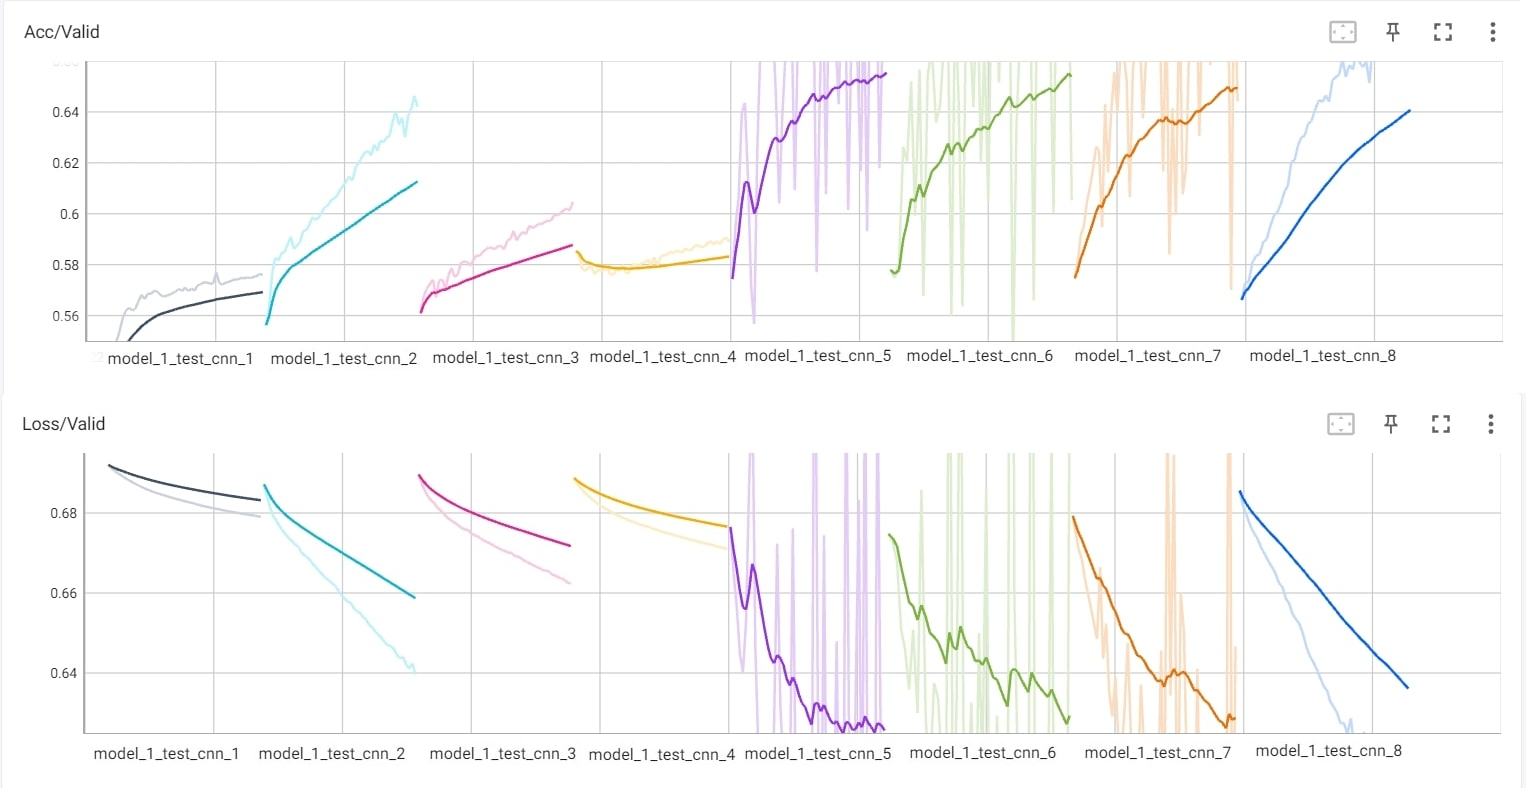
\includegraphics[width=\textwidth]{images/exp1_acc1+loss1.jpg}
        \label{fig:exp1_model1}
        \caption{Results for Model 1 at different learning rates}
    \end{figure}
\end{center}



\subsubsection{Model 2}

% Model arhitecture :
% \begin{lstlisting}[language=Python]
%     class MLP(nn.Module):
%       def __init__(self):
%         super().__init__()
%         self.layer1 = nn.Linear(768, 256)
%         self.layer2 = nn.Linear(256, 2)
%         self.activation = nn.ReLU()
%         self.drop = nn.Dropout1d(p=0.1)
%       def forward(self, x):
%         out = self.activation(self.layer1(x))
%         out = self.drop(out)
%         out = self.layer2(out)
%         return out
% \end{lstlisting}

Model 2 is also a multi-layer perceptron (MLP) with dropout regularization implemented using PyTorch's nn.Module class.

The MLP is similar to the previous model. The input to the model is expected to have a size of 768.

In addition to the previous model, this model also includes a dropout layer (self.drop) with a probability $p=0.1$. This particular layer randomly sets to 0 a fraction of input units uring training, this particular layer sets arbitrarily to 0 a portion of input units, thereby preventing overfitting by diminishing the dependence on specific neurons.


% In addition to the layers and activation function, this model also includes a dropout layer (self.drop). Dropout is a regularization technique that randomly sets a fraction of input units to 0 during training, which helps prevent overfitting by reducing the reliance on specific neurons.

% In the initialization method (\_\_init\_\_), the architecture is defined with the same linear layers as before, and the ReLU activation function is applied between the layers. Additionally, a dropout layer with a dropout rate of 0.1 is added.

% In the forward method, the input x is passed through the layers of the model. After the first linear layer and activation function, the output is passed through the dropout layer (self.drop) before proceeding to the second linear layer. The dropout layer randomly sets a fraction of the activations to 0, promoting the model's robustness by reducing over-dependence on specific activations.

% The final output of the model represents the predicted class probabilities for a binary classification task, as in the previous model.

In summary, this model extends the previous MLP by incorporating dropout regularization.

\begin{center}
    \begin{figure}[!ht]
        \centering
        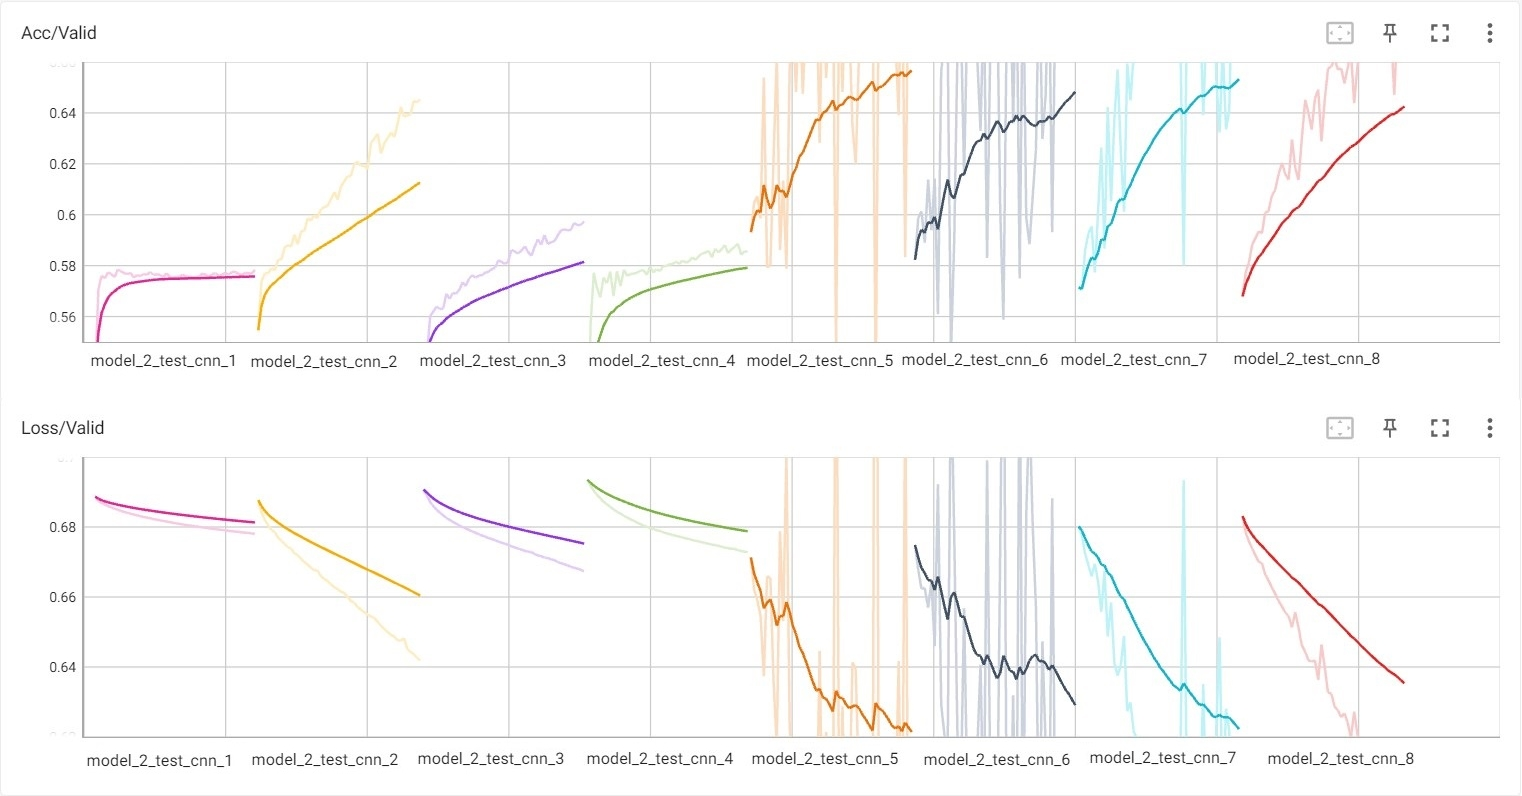
\includegraphics[width=\textwidth]{images/exp1_acc2+loss2.jpg}
        \label{fig:exp1_model2}
        \caption{Results for Model 2 at different learning rates}
    \end{figure}
\end{center}


\subsubsection{Model 3}

% Model arhitecture :
% \begin{lstlisting}[language=Python]
%     class MLP(nn.Module):
%       def __init__(self):
%         super().__init__()
%         self.layer1 = nn.Linear(768, 256)
%         self.layer2 = nn.Linear(256, 2)
%         self.activation = nn.Tanh()
%         self.drop = nn.Dropout1d(p=0.1)
%       def forward(self, x):
%         out = self.activation(self.layer1(x))
%         out = self.drop(out)
%         out = self.layer2(out)
%         return out
% \end{lstlisting}

Model 3 is a multi-layer perceptron (MLP) with dropout regularization and a hyperbolic tangent activation function implemented using PyTorch's nn.Module class. Tanh is an activation function used on each layer 1 output. This can be observed in the following chart:

% However, instead of using the ReLU activation function, this model utilizes the hyperbolic tangent (Tanh) activation function (self.activation). The Tanh activation function maps the input values to the range [-1, 1], allowing for non-linear transformations.

% Similar to the previous models, this MLP has two hidden layers and one output layer. The input to the model is expected to have a size of 768.

% In the initialization method (\_\_init\_\_), the architecture is defined with the same linear layers as before. 

% However, instead of using the ReLU activation function, this model utilizes the hyperbolic tangent (Tanh) activation function (self.activation). The Tanh activation function maps the input values to the range [-1, 1], allowing for non-linear transformations.

% Additionally, a dropout layer with a dropout rate of 0.1 is included (self.drop). Dropout regularization randomly sets a fraction of input units to 0 during training, reducing overfitting and improving generalization.

% In the forward method, the input x is passed through the layers of the model. After the first linear layer and Tanh activation function, the output is passed through the dropout layer (self.drop). Finally, the output from the dropout layer is fed into the second linear layer to produce the final output of the model.

% The output of the model represents the predicted class probabilities for a binary classification task, as in the previous models.

% In summary, this model is an MLP with two hidden layers, dropout regularization, and a hyperbolic tangent activation function. The Tanh activation function allows for non-linear transformations, while dropout regularization helps prevent overfitting.

\begin{center}
    \begin{figure}[!ht]
        \centering
        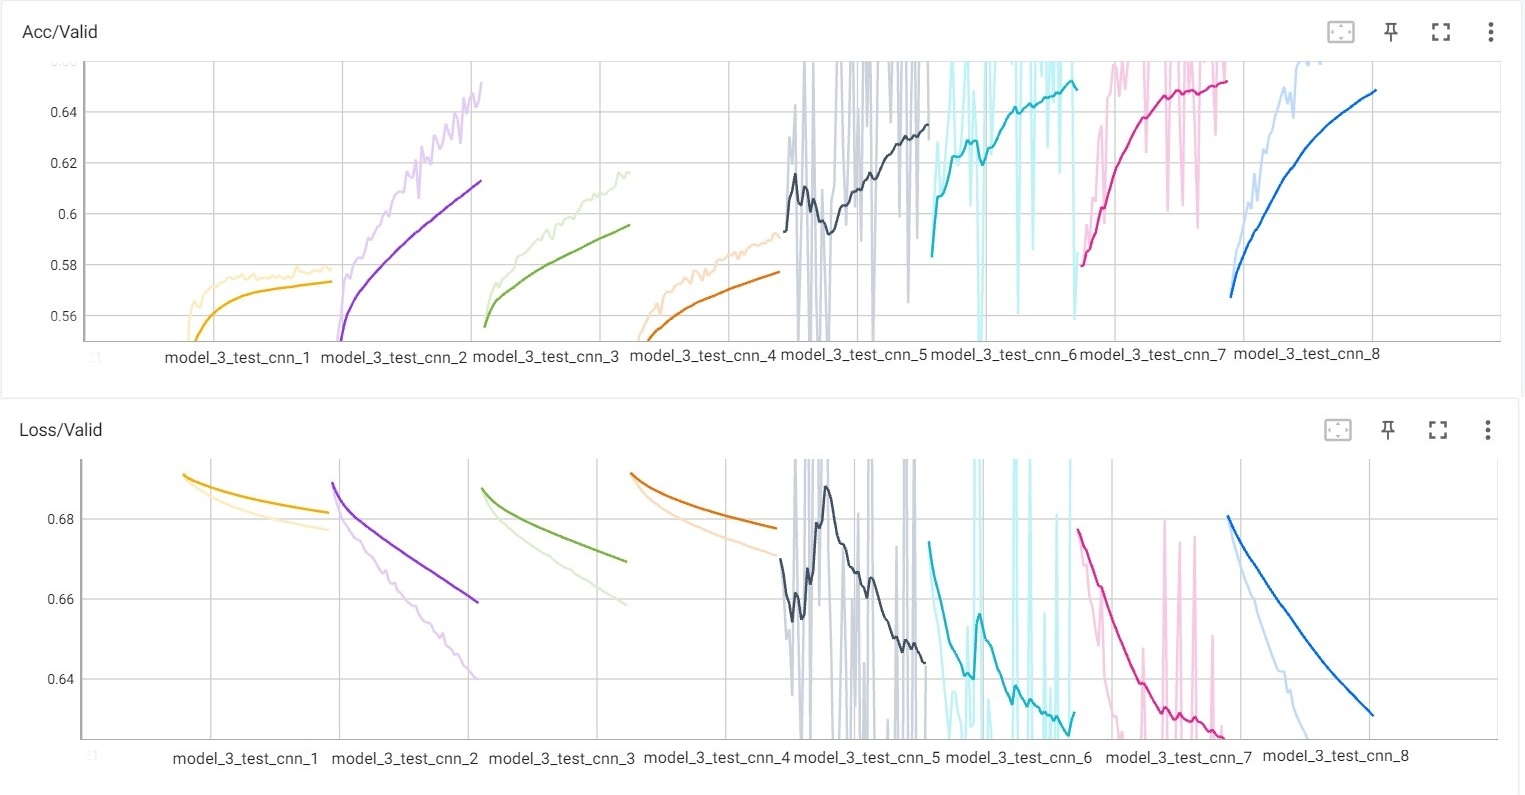
\includegraphics[width=\textwidth]{images/exp1_acc3+loss3.jpg}
        \label{fig:exp1_model3}
        \caption{Results for Model 3 at different learning rates}
    \end{figure}
\end{center}



\subsubsection{Model 4}

% Model arhitecture :
% \begin{lstlisting}[language=Python]
%     class MLP(nn.Module):
%       def __init__(self):
%         super().__init__()
%         self.layer1 = nn.Linear(768, 512)
%         self.layer2 = nn.Linear(512, 128)
%         self.layer3 = nn.Linear(128, 2)
%         self.activation = nn.ReLU()
%       def forward(self, x):
%         out = self.activation(self.layer1(x))
%         out = self.layer2(out)
%         out = self.layer3(out)
%         return out
% \end{lstlisting}

The model described in the code snippet is a multi-layer perceptron (MLP) with three hidden layers implemented using PyTorch's nn.Module class. It is similar to model 1, with the main difference consisting of it having only 3 layers instead of 3. Their dimensionality is set off at 768 and then merged at 512, 128 and 2 respectively. The results are shown in the table below:

% This MLP architecture is designed for a binary classification task. The input to the model is expected to have a size of 768.

% In the initialization method (\_\_init\_\_), the model's architecture is defined. It consists of three linear layers (self.layer1, self.layer2, and self.layer3) with 512, 128, and 2 units, respectively. Each linear layer represents a fully connected layer, where each neuron is connected to every neuron in the previous layer. The first linear layer takes the input of size 768 and outputs a tensor of size 512. The second linear layer takes the output of the previous layer (512) and outputs a tensor of size 128. Finally, the third linear layer takes the output of the second layer (128) and produces a tensor of size 2, representing the predicted class probabilities for the binary classification task.

% The ReLU activation function (self.activation) is applied between the first and second layers. ReLU (Rectified Linear Unit) is a commonly used activation function that introduces non-linearity into the model by setting negative values to zero and keeping positive values unchanged.

% In the forward method, the input x is passed through the layers of the model. First, the input is passed through the first linear layer (self.layer1) and then through the activation function (self.activation) which applies the ReLU activation element-wise. The resulting tensor is then passed through the second and third linear layers without an intermediate activation function.

% Overall, the model architecture described in the code snippet is an MLP with three hidden layers and ReLU activation function. It takes an input of size 768, processes it through the layers, and produces the final output of size 2 for the binary classification task.

\begin{center}
    \begin{figure}[!ht]
        \centering
        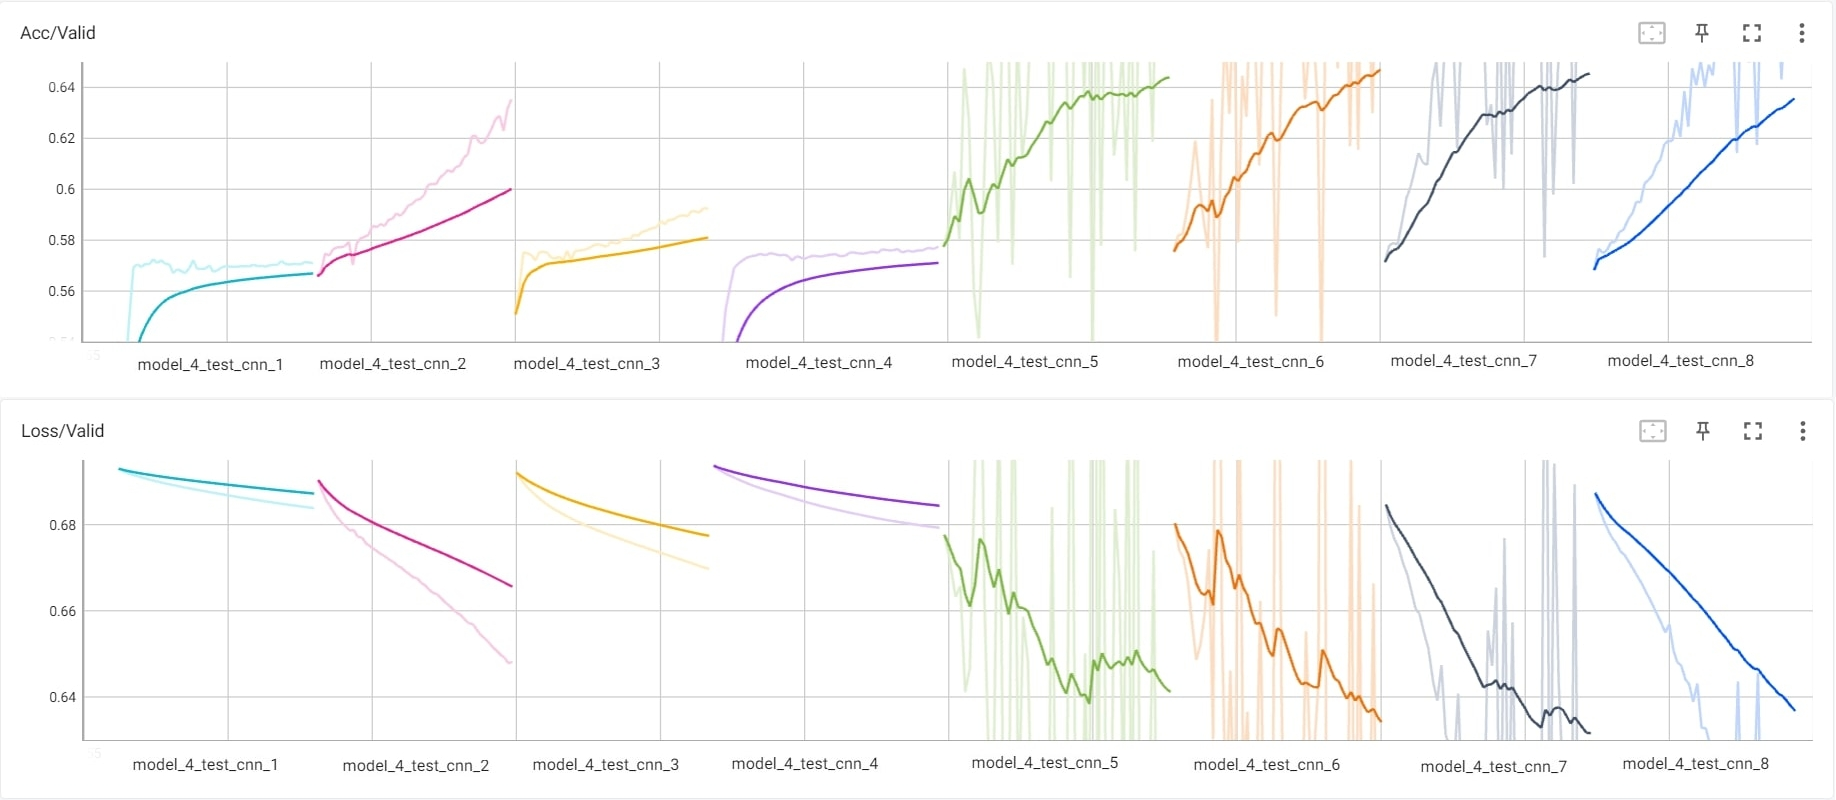
\includegraphics[width=\textwidth]{images/exp1_acc4+loss4.jpg}
        \label{fig:exp1_model4}
        \caption{Results for Model 4 at different learning rates}
    \end{figure}
\end{center}

\subsubsection{Model 5}

% Model arhitecture :
% \begin{lstlisting}[language=Python]
%     class MLP(nn.Module):
%       def __init__(self):
%         super().__init__()
%         self.layer1 = nn.MaxPool1d(3, stride=2)
%         self.layer2 = nn.Linear(383, 128)
%         self.layer3 = nn.Linear(128, 2)
%         self.activation = nn.Tanh()
%         self.drop = nn.Dropout1d(p=0.1)
%       def forward(self, x):
%         out = self.activation(self.layer1(x))
%         out = self.layer2(out)
%         out = self.drop(out)
%         out = self.layer3(out)
%         return out
% \end{lstlisting}

The model described in the code snippet is a multi-layer perceptron (MLP) with max pooling, dropout regularization, and a hyperbolic tangent activation function implemented using PyTorch's nn.Module class. Model 5 is similar to model 3. The difference consists in adding a maxpool1d layer before the first linear layer. The results are shown in the table below:

% This MLP architecture is designed for a binary classification task. The input to the model is expected to have a size that allows for max pooling.

% In the initialization method (\_\_init\_\_), the model's architecture is defined. It consists of a max pooling layer (self.layer1) with a kernel size of 3 and a stride of 2, which reduces the spatial dimensions of the input. Following the max pooling layer, there are two linear layers (self.layer2 and self.layer3) with 128 and 2 units, respectively. Each linear layer represents a fully connected layer, where each neuron is connected to every neuron in the previous layer.

% The hyperbolic tangent (Tanh) activation function (self.activation) is applied after the max pooling layer and the first linear layer. The Tanh activation function maps the input values to the range [-1, 1].

% In addition, a dropout layer with a dropout rate of 0.1 is included (self.drop). Dropout regularization randomly sets a fraction of input units to 0 during training, reducing overfitting and improving generalization.

% In the forward method, the input x is passed through the layers of the model. The input first goes through the max pooling layer (self.layer1), followed by the hyperbolic tangent activation function (self.activation). Then, the output is passed through the second linear layer (self.layer2). After that, dropout is applied to the output using self.drop. Finally, the output from the dropout layer is fed into the third linear layer (self.layer3) to produce the final output of the model.

% The output of the model represents the predicted class probabilities for a binary classification task.

% In summary, this model is an MLP with max pooling, dropout regularization, and a hyperbolic tangent activation function. The max pooling layer reduces the spatial dimensions, the dropout layer helps prevent overfitting, and the hyperbolic tangent activation function allows for non-linear transformations.

\begin{center}
    \begin{figure}[!h]
        \centering
        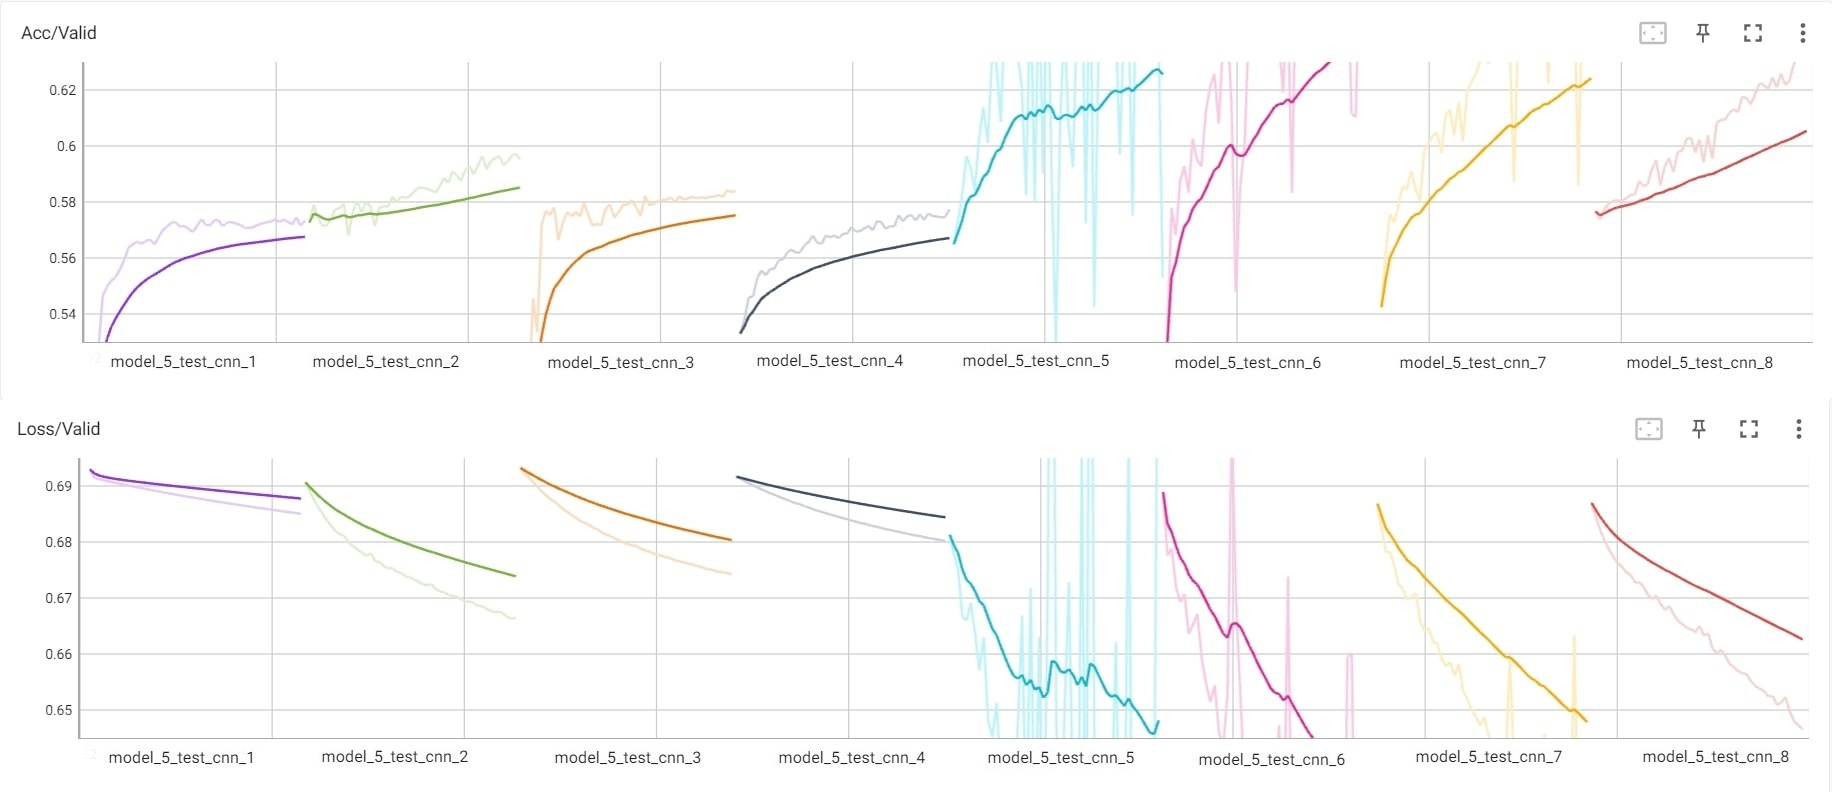
\includegraphics[width=\textwidth]{images/exp1_acc5+loss5.jpg}
        \label{fig:exp1_model5}
        \caption{Results for Model 5 at different learning rates}
    \end{figure}
\end{center}

\subsubsection{Model 6}

% Model arhitecture :
% \begin{lstlisting}[language=Python]
%     class MLP(nn.Module):
%       def __init__(self):
%         super().__init__()
%         self.layer1 = nn.MaxPool1d(3, stride=2)
%         self.layer2 = nn.Linear(383, 128)
%         self.layer3 = nn.Linear(128, 2)
%         self.activation = nn.RReLU()
%         self.drop = nn.Dropout1d(p=0.15)
%       def forward(self, x):
%         out = self.activation(self.layer1(x))
%         out = self.layer2(out)
%         out = self.drop(out)
%         out = self.layer3(out)
%         return out
% \end{lstlisting}

The model described in the code snippet is a multi-layer perceptron (MLP) with max pooling, dropout regularization, and a randomized leaky rectified linear unit (RReLU) activation function implemented using PyTorch's nn.Module class. Based on model 5 we changed the activation function from tanh to relu. Also, the dropout probability was raised from 0.1 to 0.5. The results are presented in the graph below:

% This MLP architecture is designed for a binary classification task. The input to the model is expected to have a size that allows for max pooling.

% In the initialization method (\_\_init\_\_), the model's architecture is defined. It consists of a max pooling layer (self.layer1) with a kernel size of 3 and a stride of 2, which reduces the spatial dimensions of the input. Following the max pooling layer, there are two linear layers (self.layer2 and self.layer3) with 128 and 2 units, respectively. Each linear layer represents a fully connected layer, where each neuron is connected to every neuron in the previous layer.

% The randomized leaky rectified linear unit (RReLU) activation function (self.activation) is applied after the max pooling layer and the first linear layer. RReLU is a variant of the rectified linear unit (ReLU) activation function that introduces a random component to the negative range, allowing for potential learning even when the input is negative.

% In addition, a dropout layer with a dropout rate of 0.15 is included (self.drop). Dropout regularization randomly sets a fraction of input units to 0 during training, reducing overfitting and improving generalization.

% In the forward method, the input x is passed through the layers of the model. The input first goes through the max pooling layer (self.layer1), followed by the RReLU activation function (self.activation). Then, the output is passed through the second linear layer (self.layer2). After that, dropout is applied to the output using self.drop. Finally, the output from the dropout layer is fed into the third linear layer (self.layer3) to produce the final output of the model.

% The output of the model represents the predicted class probabilities for a binary classification task.

% In summary, this model is an MLP with max pooling, dropout regularization, and a randomized leaky rectified linear unit (RReLU) activation function. The max pooling layer reduces the spatial dimensions, the dropout layer helps prevent overfitting, and the RReLU activation function introduces randomness to negative inputs, potentially aiding learning.


\begin{center}
    \begin{figure}[!h]
        \centering
        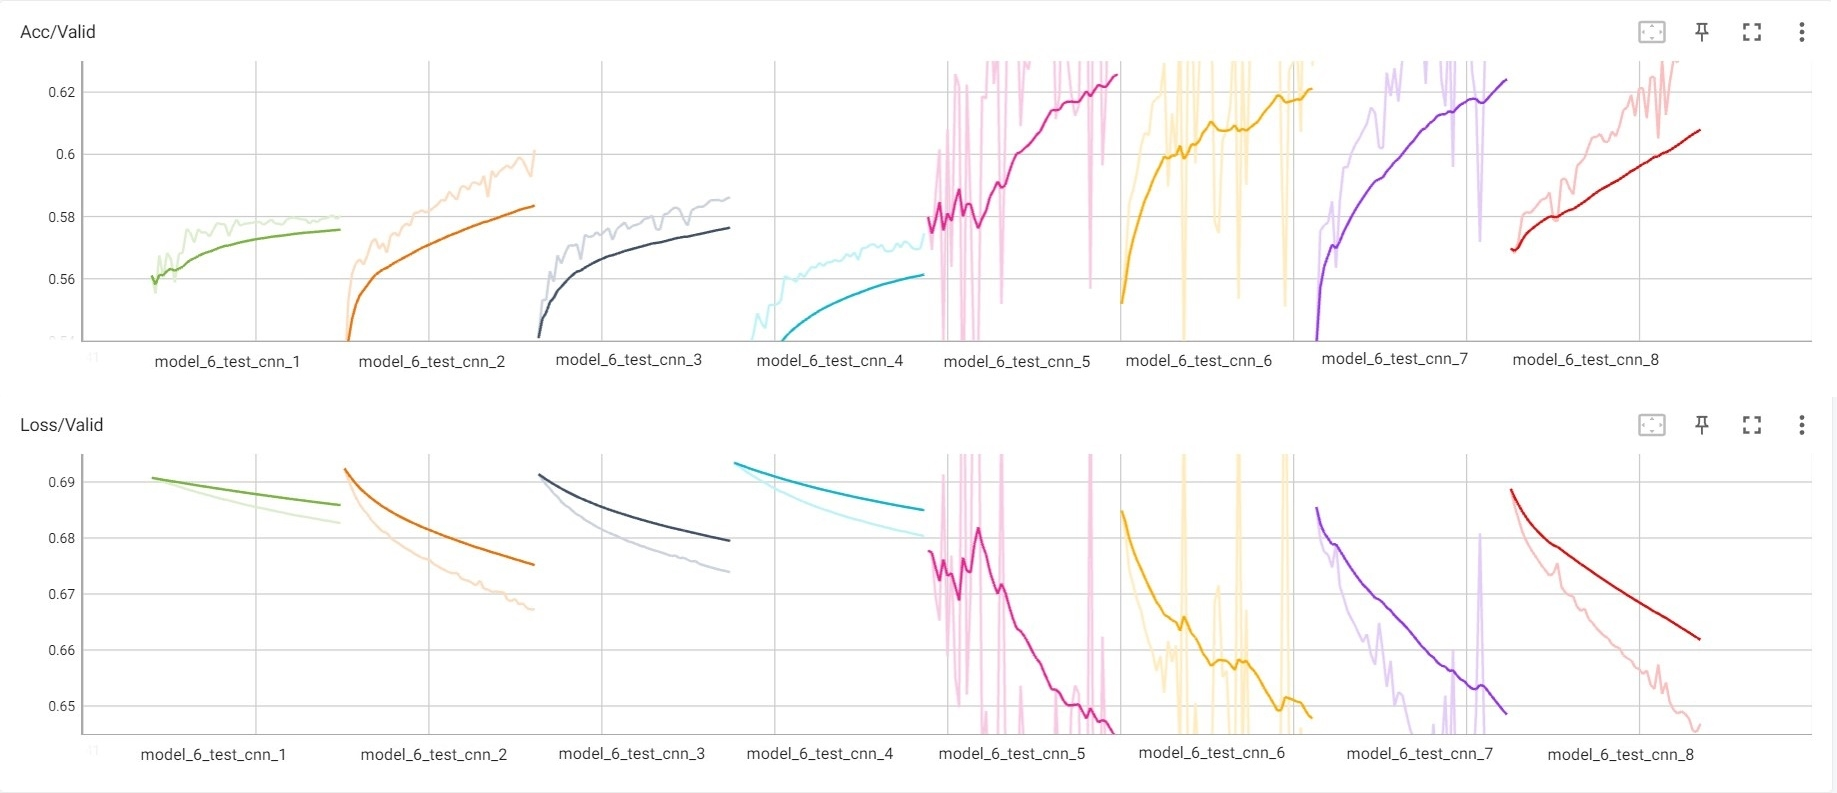
\includegraphics[width=\textwidth]{images/exp1_acc6+loss6.jpg}
        \label{fig:exp1_model6}
        \caption{Results for Model 6 at different learning rates}
    \end{figure}
\end{center}


\subsubsection{Comparation}
\begin{center}
    \begin{tabular}{|p{3cm}||p{3cm}|p{3cm}|  }
     % \hline
     % \multicolumn{3}{|c|}{BERT fine-tunning results} \\
     \hline
    Model number	& Accuracy & Loss \\
     \hline
    Model 1 & 71.07\% & 0.5611\\
    \textbf{Model 2} & \textbf{71.23}\% & 0.5691\\
    \textbf{Model 3} & \textbf{71.4}\% & 0.5682\\
    \textbf{Model 4} & \textbf{71.42}\% & 0.5611\\
    Model 5 & 68.58\% & 0.5994\\
    Model 6 & 69.03\% & 0.6034\\
     \hline
    \end{tabular}
    \captionof{table}{BERT fine-tunning results: Experiment 1}
\end{center}

As already noticed, models 2, 3 and 4 had high accuracy, so we will use them to do fine tuning when we retrain the BERT model as well.

\begin{center}
    \begin{figure}[!h]
        \centering
        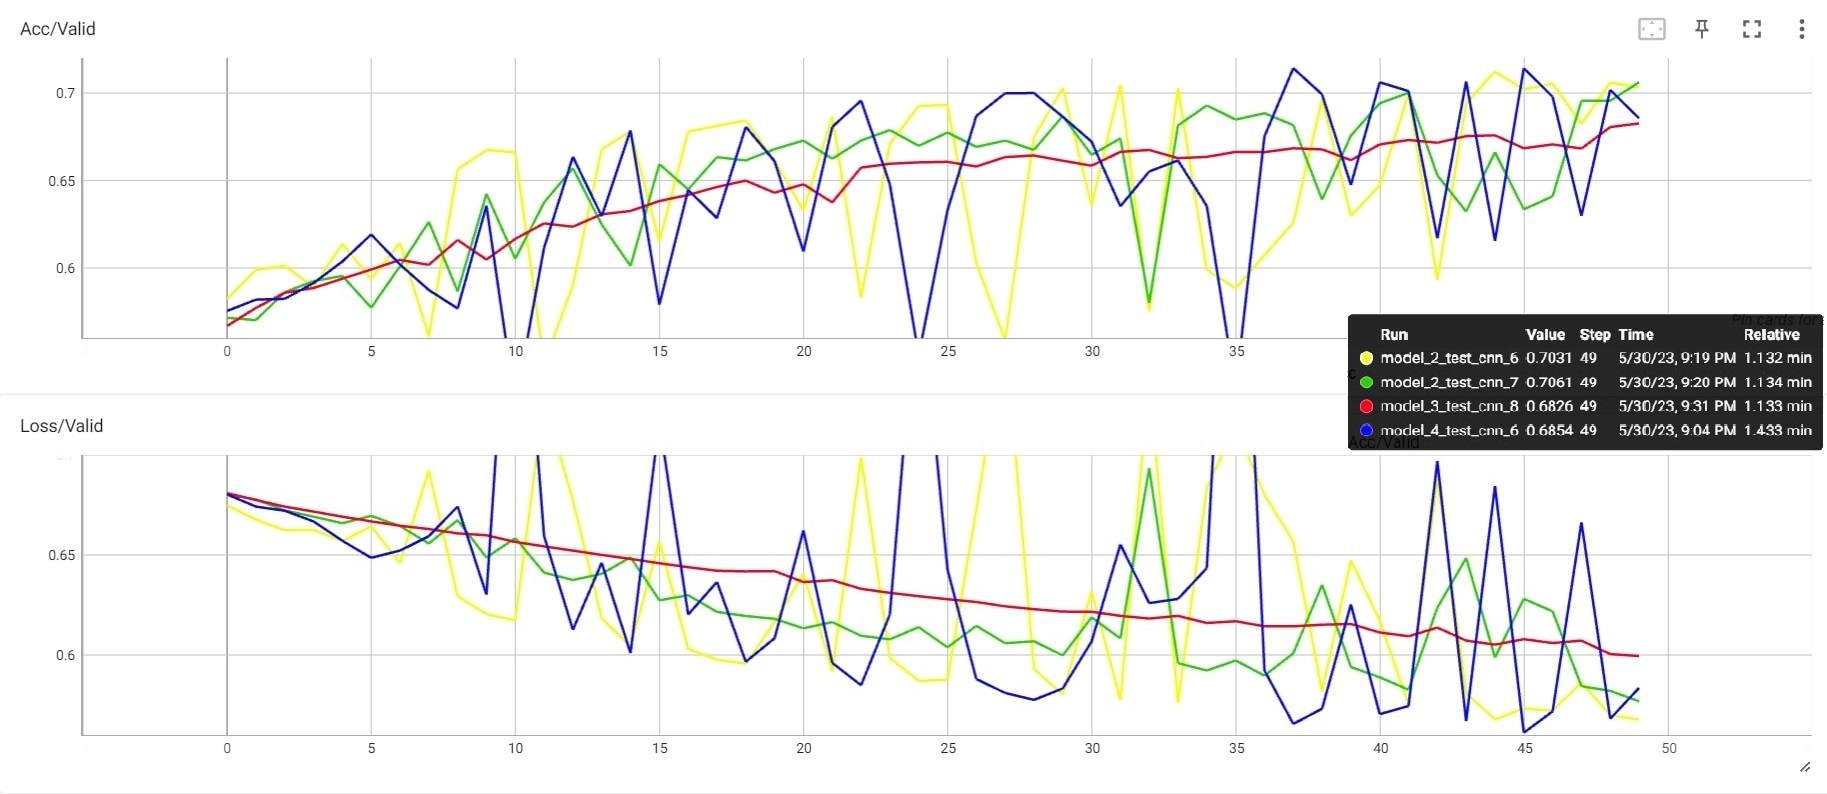
\includegraphics[width=\textwidth]{images/exp1_hiperparametrizare.jpg}
        \label{fig:exp1_hiperm}
        \caption{Results for Model 2, 3 and 4}
    \end{figure}
\end{center}

\subsection{Experiment 2}

In experiment 2, I took Models 2, 3 and 4 and redefined the Neural Network class to retrain with BERT. The learning rate took the values: $4*10^{-5}, 2*10^{-5}$. The batch size was kept at 32.

\subsubsection{Model 2}

Code for this model defines a PyTorch module called MLP that incorporates a BERT model as part of its architecture. The BERT model is passed as a parameter mod to the \_\_init\_\_ method. Here's a breakdown of the model's components and functionality:

\begin{itemize}
    \item self.bert = mod: This line assigns the BERT model received in the mod variable to the self.bert attribute of the MLP class.
    \item self.layer1 = nn.Linear(768, 256): This creates a linear layer with an input size of 768 and an output size of 256. It is the first layer after the BERT model.
    \item self.layer2 = nn.Linear(256, 2): This creates another linear layer with an input size of 256 and an output size of 2. It is the second and final layer of the MLP.
    \item self.activation = nn.ReLU(): This defines the activation function to be applied after the first linear layer. In this case, it uses the Rectified Linear Unit (ReLU) activation function.
    \item self.drop = nn.Dropout1d(p=0.1): This creates a dropout layer with a dropout rate of 0.1. 
\end{itemize}

The forward method of the MLP class implements the forward pass of the model. Here's a breakdown of its steps:
\begin{itemize}
    \item out = self.bert(ids, attention\_mask=mask, token\_type\_ids=token\_type\_ids) \newline ['pooler\_output']: This line applies the BERT model to the input ids, mask, and token\_type\_ids. It retrieves the 'pooler\_output' from the BERT model's output dictionary. The 'pooler\_output' typically represents a fixed-size representation of the entire input sequence.

    \item out = self.activation(out): tensor is passed through the activation function. In this case, it uses the ReLU activation function. This line is tested both : commented, which means that BERT output is not activated - Model 2A, and not commented, which means that BERT output is activated - Model 2B.

    \item out = self.activation(self.layer1(out)): The out tensor is passed through the first linear layer and then activated using the ReLU activation function.

    \item out = self.drop(out): Dropout is applied to the output of the first linear layer.

    \item out = self.layer2(out): The output from the dropout layer is passed through the second linear layer.

    \item return out: The final output of the MLP is returned.
\end{itemize}

In summary, this MLP class integrates a BERT model as a component of its architecture and applies a two-layer feed-forward neural network on top of the BERT output to perform a specific task, which is not evident from the provided code.

\begin{center}
    \begin{figure}[!h]
        \centering
        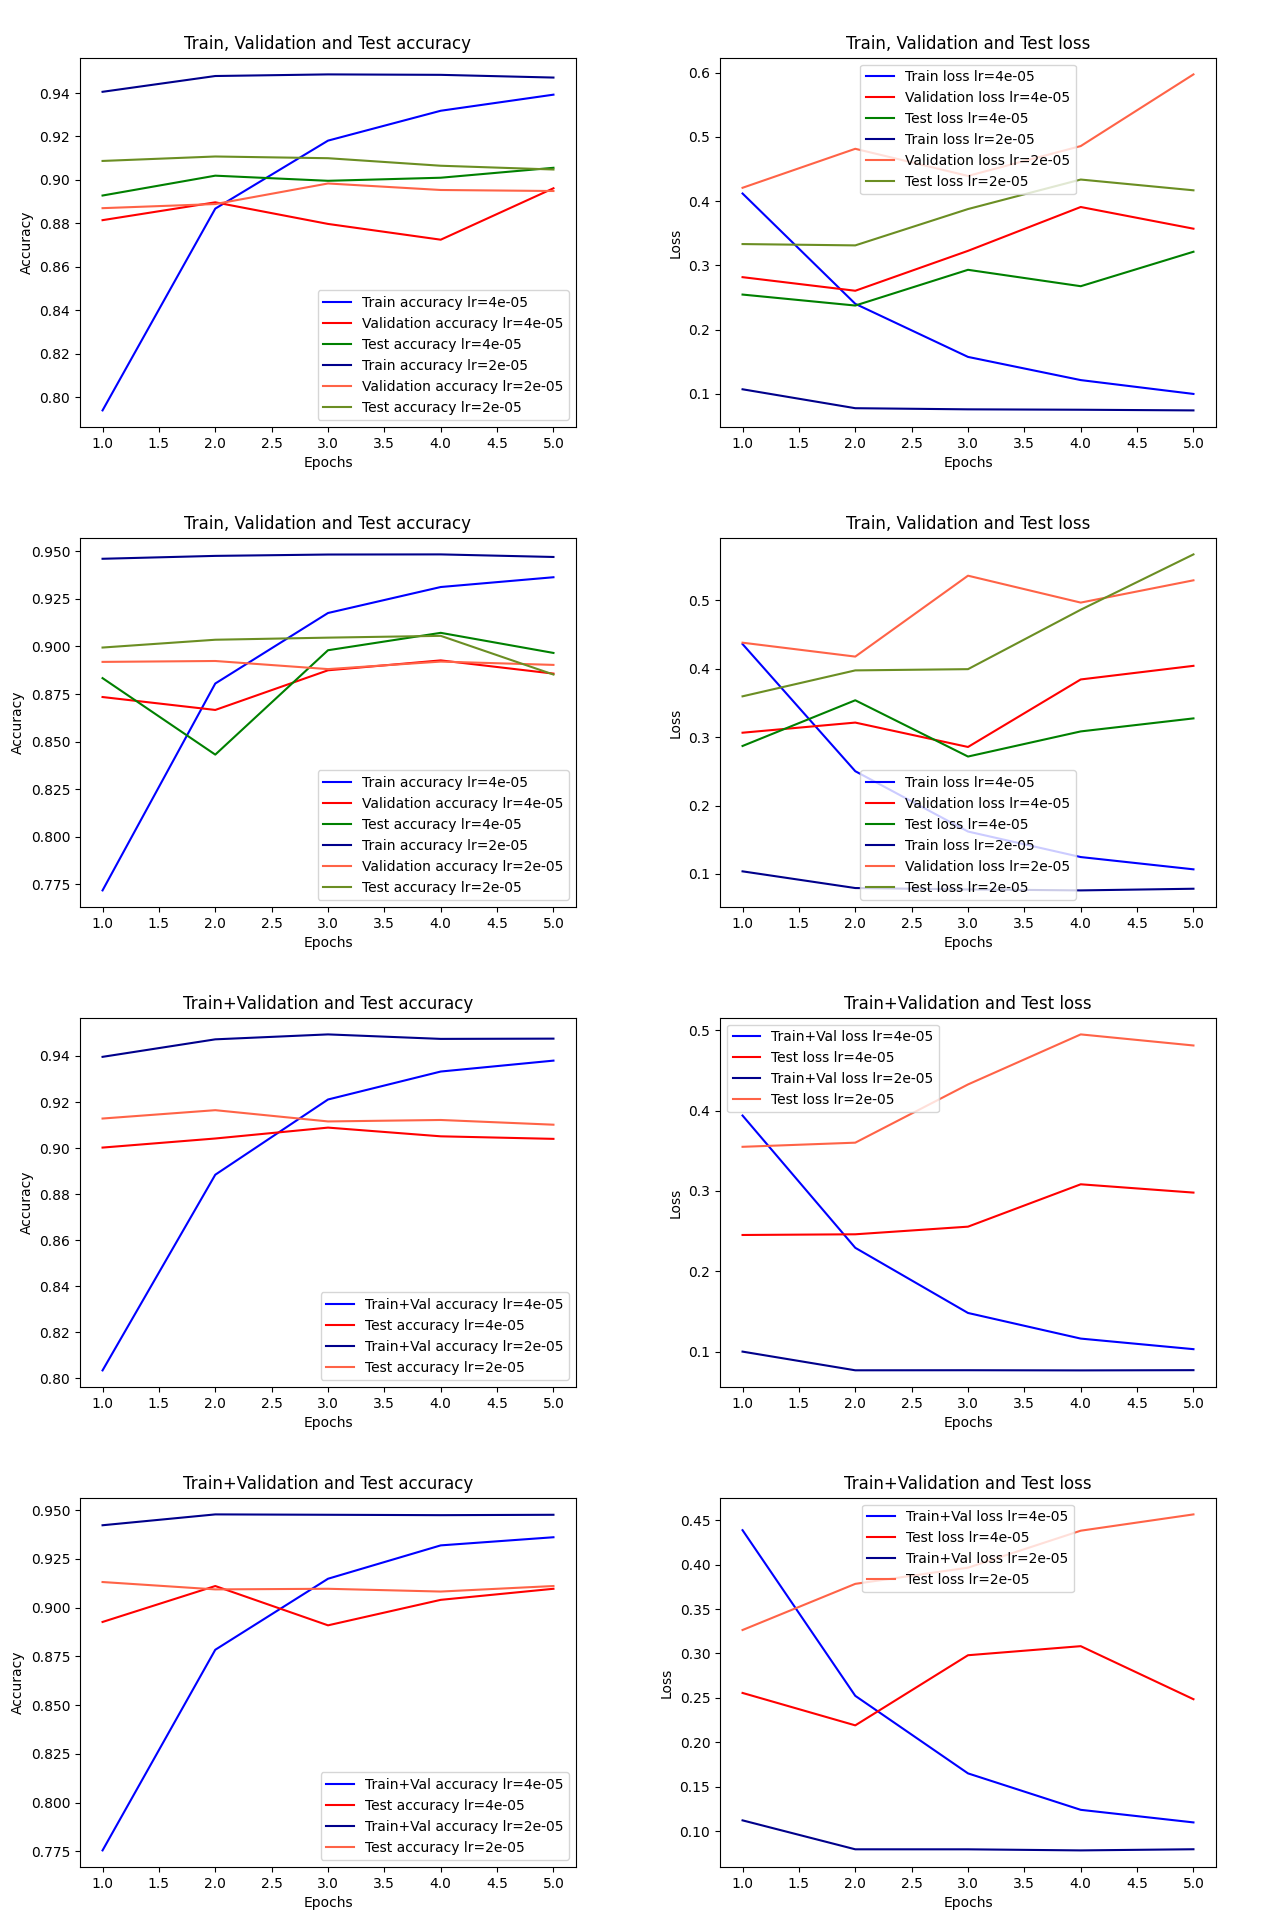
\includegraphics[width=0.8\textwidth]{images/ger_model1_vertical.png}
        \label{fig:ger_model1}
        \caption{Results for Model 2 with and without BERT activation. Tested on Validation(top half) and on Test(bottom half)}
    \end{figure}
\end{center}


\subsubsection{Model 3}

Code for this model defines a PyTorch module called MLP that incorporates a BERT model as part of its architecture. The BERT model is passed as a parameter mod to the \_\_init\_\_ method. Here's a breakdown of the model's components and functionality:

\begin{itemize}
    \item self.bert = mod: This line assigns the BERT model received in the mod variable to the self.bert attribute of the MLP class.

    \item self.layer1 = nn.Linear(768, 256): This creates a linear layer with an input size of 768 and an output size of 256. It is the first layer after the BERT model.

    \item self.layer2 = nn.Linear(256, 2): This creates another linear layer with an input size of 256 and an output size of 2. It is the second and final layer of the MLP.

    \item self.activation = nn.Tanh(): This defines the activation function to be applied after the BERT output and the first linear layer. In this case, it uses the hyperbolic tangent (Tanh) activation function.

    \item self.drop = nn.Dropout1d(p=0.1): This creates a dropout layer with a dropout rate of 0.1. Dropout is applied to prevent wrongly classifying certain data as important by unsystematically positioning a fraction of the input elements to zero in the training process.
    
\end{itemize}


The forward method of the MLP class implements the forward pass of the model. Here's a breakdown of its steps:

\begin{itemize}
    \item out = self.bert(ids, attention\_mask=mask, token\_type\_ids=token\_type\_ids) \newline ['pooler\_output']: This line applies the BERT model to the input ids, mask, and token\_type\_ids. It retrieves the 'pooler\_output' from the BERT model's output dictionary. The 'pooler\_output' typically represents a fixed-size representation of the entire input sequence.

    \item out = self.activation(out): The out tensor is passed through the activation function, which is the hyperbolic tangent (Tanh) in this case. This line is tested both : commented, which means that BERT output is not activated - Model 3A, and not commented, which means that BERT output is activated - Model 3B.

    \item out = self.activation(self.layer1(out)): The output from the previous activation function is passed through the first linear layer and then activated using the Tanh activation function again.

    \item out = self.drop(out): Dropout is applied to the output of the first linear layer.

    \item out = self.layer2(out): The output from the dropout layer is passed through the second linear layer.

    \item return out: The final output of the MLP is returned.
\end{itemize}

In summary, this MLP class integrates a BERT model as a component of its architecture and applies a two-layer feed-forward neural network on top of the BERT output. The activation function used in this model is the hyperbolic tangent (Tanh). Dropout is applied to the output of the first linear layer to prevent overfitting.

\begin{center}
    \begin{figure}[!h]
        \centering
        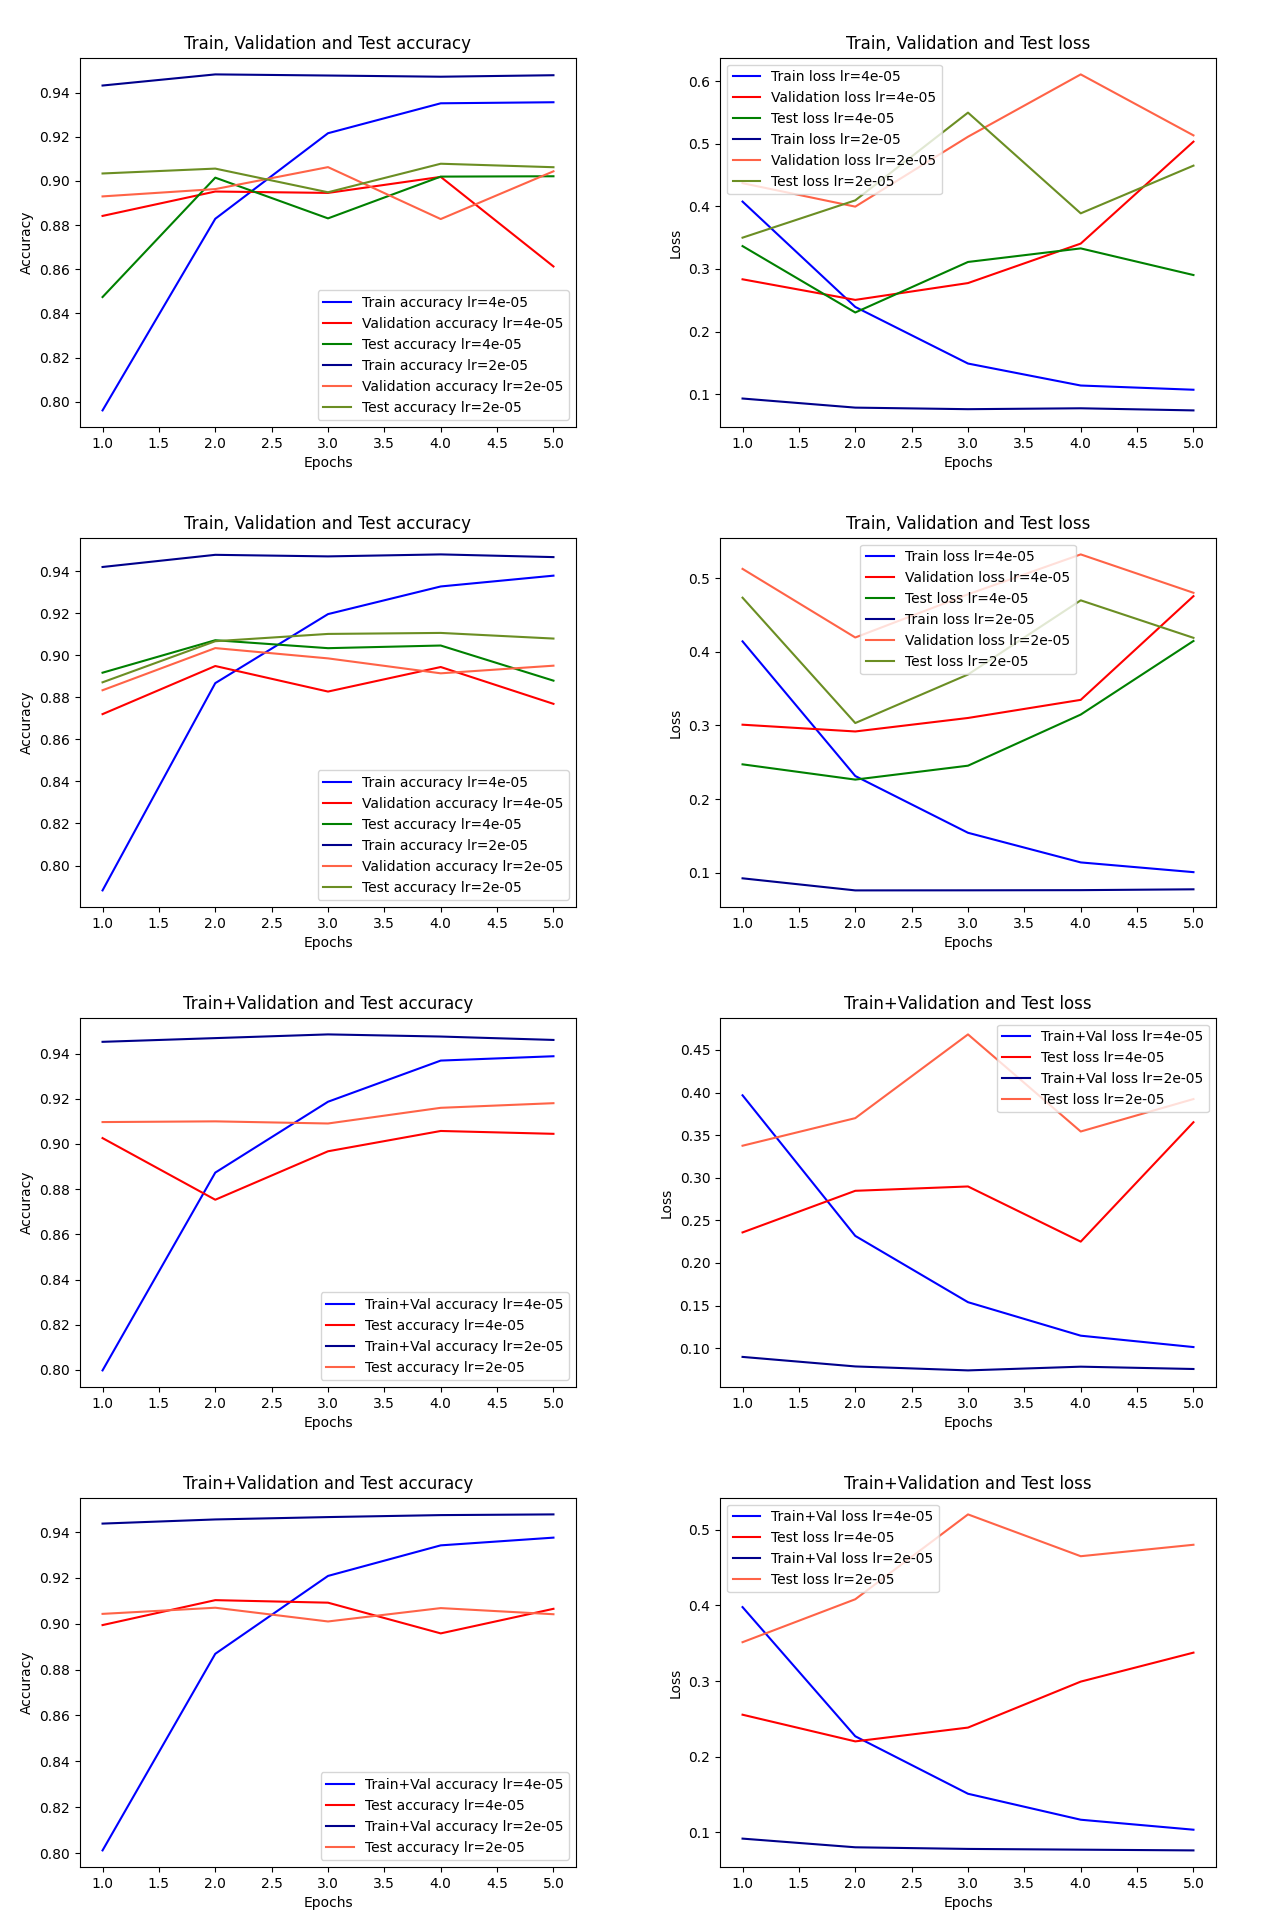
\includegraphics[width=0.8\textwidth]{images/ger_model2_vertical.png}
        \label{fig:ger_model2}
        \caption{Results for Model 3 with and without BERT activation. Tested on Validation(top half) and on Test(bottom half)}
    \end{figure}
\end{center}


\subsubsection{Model 4}

Code for this model defines a PyTorch module called MLP that incorporates a BERT model as part of its architecture. The BERT model is passed as a parameter mod to the \_\_init\_\_ method. Here's a breakdown of the model's components and functionality:

\begin{itemize}
    \item self.bert = mod: This line assigns the BERT model received in the mod variable to the self.bert attribute of the MLP class.

    \item self.layer1 = nn.Linear(768, 512): This creates a linear layer with an input size of 768 (the output size of the BERT model) and an output size of 512.

    \item self.layer2 = nn.Linear(512, 128): This creates another linear layer with an input size of 512 and an output size of 128.

    \item self.layer3 = nn.Linear(128, 2): This creates the final linear layer with an input size of 128 and an output size of 2.

    \item self.activation = nn.ReLU(): This defines the activation function to be applied after each linear layer. In this case, it uses the Rectified Linear Unit (ReLU) activation function.
\end{itemize}

The forward method of the MLP class implements the forward pass of the model. Here's a breakdown of its steps:

\begin{itemize}
    \item out = self.bert(ids, attention\_mask=mask, token\_type\_ids=token\_type\_ids) \newline ['pooler\_output']: This line applies the BERT model to the input ids, mask, and token\_type\_ids. It retrieves the 'pooler\_output' from the BERT model's output dictionary. The 'pooler\_output' typically represents a fixed-size representation of the entire input sequence.

    \item out = self.activation(out): The out tensor is passed through the activation function, which is the Rectified Linear Unit (ReLU) in this case. This line is tested both : commented, which means that BERT output is not activated - Model 4A, and not commented, which means that BERT output is activated - Model 4B.

    \item out = self.activation(self.layer1(out)): The output from the previous activation function is passed through the first linear layer and then activated using the ReLU activation function again.

    \item out = self.layer2(out): The output from the previous layer is passed through the second linear layer.

    \item out = self.layer3(out): The output from the previous layer is passed through the final linear layer.

    \item return out: The final output of the MLP is returned.
\end{itemize}

In summary, this MLP class integrates a BERT model as a component of its architecture and applies a three-layer feed-forward neural network on top of the BERT output. The activation function used between the linear layers is the Rectified Linear Unit (ReLU). The output of the last linear layer is returned as the final output of the MLP.

\begin{center}
    \begin{figure}[!h]
        \centering
        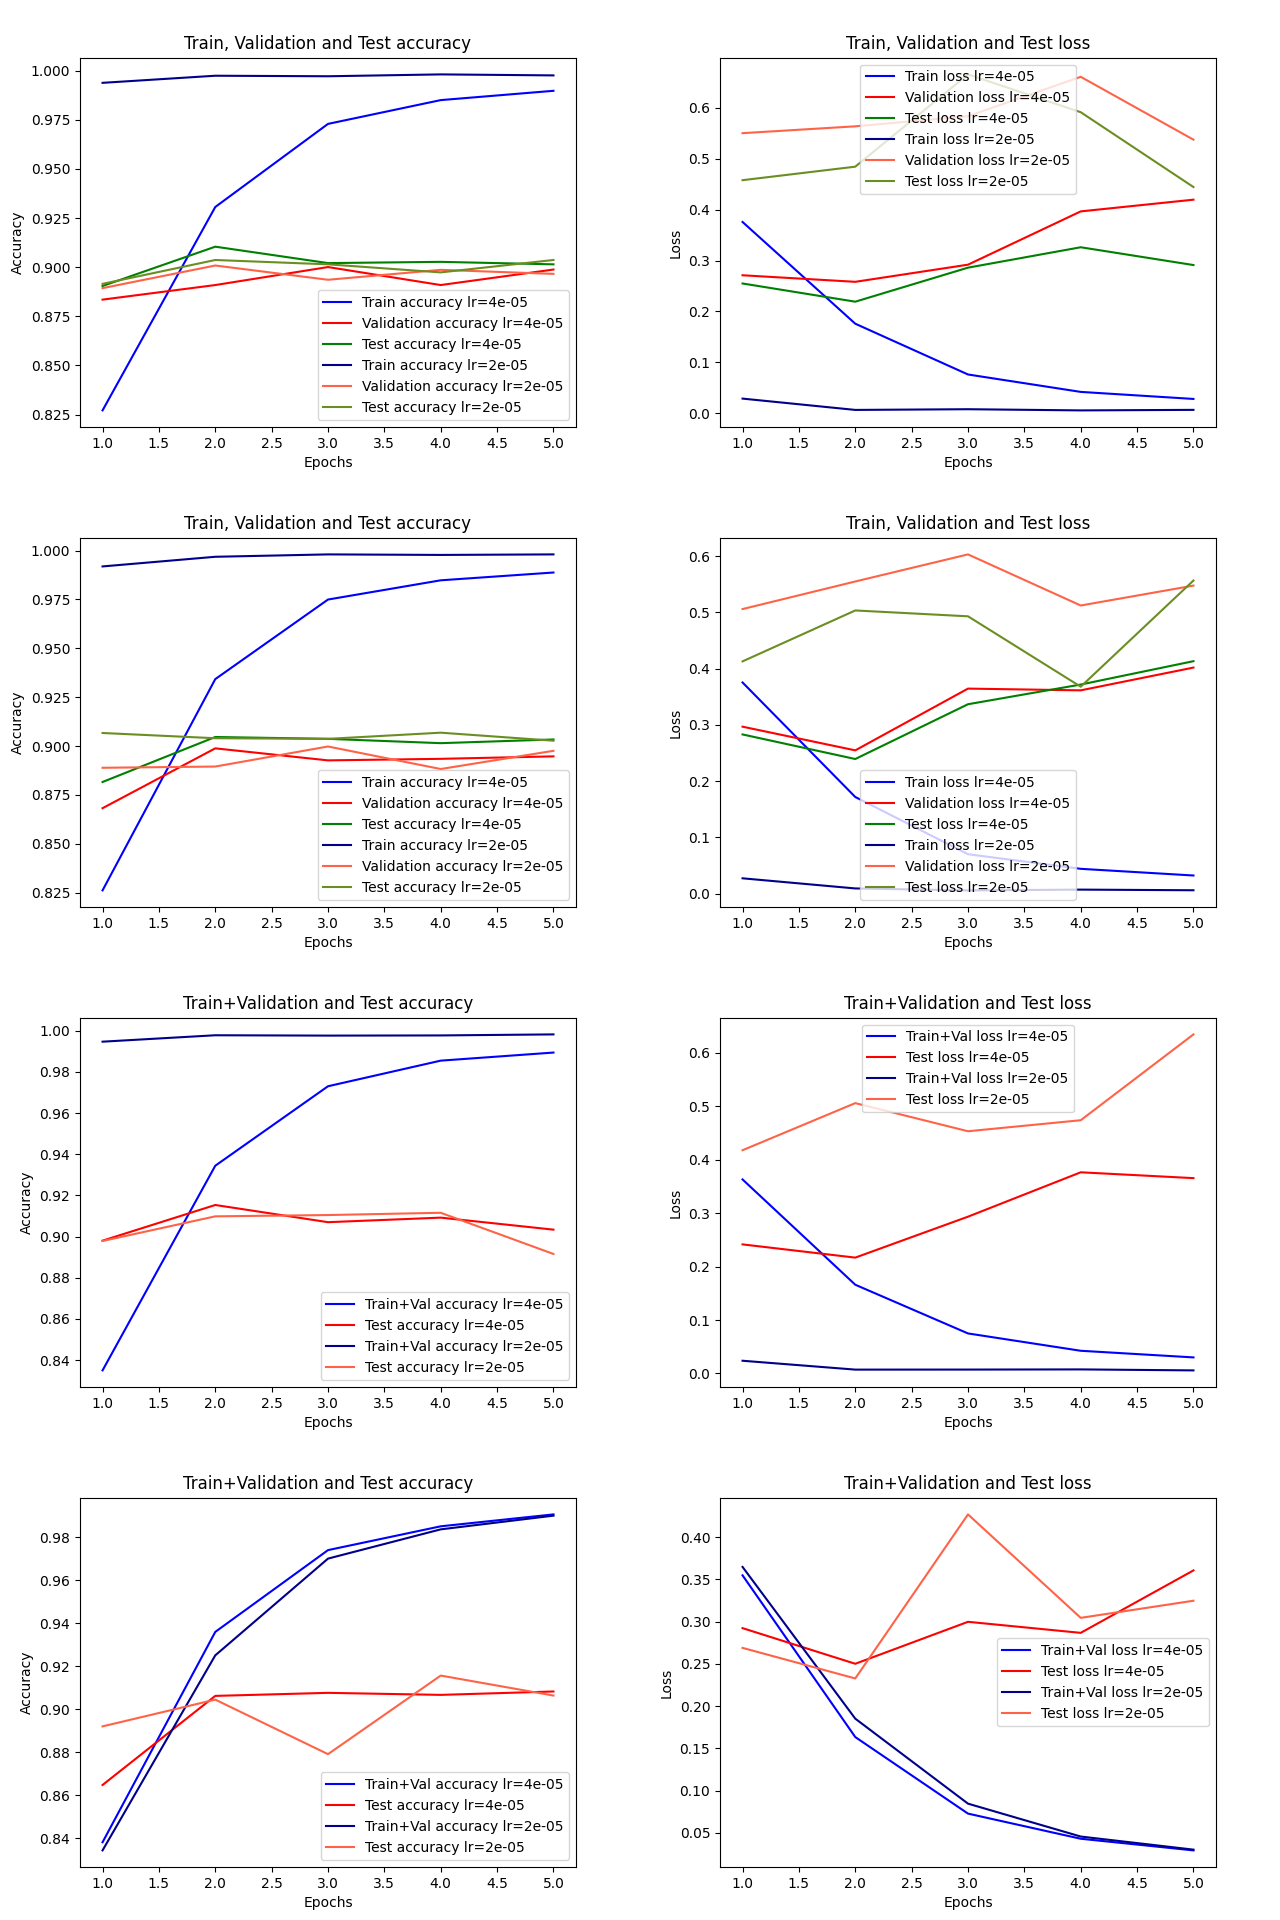
\includegraphics[width=0.8\textwidth]{images/ger_model3_vertical.png}
        \label{fig:ger_model3}
        \caption{Results for Model 4 with and without BERT activation. Tested on Validation(top half) and on Test(bottom half)}
    \end{figure}
\end{center}

